\chapter{Experimental Results}
\label{chapter6}
\hspace*{6mm}For checking and validating the proposed method, we set up experiments from technical and pre-clinical perspective. In technical perspective, admittance control, force-guided alignment, and file feedrate control were conducted and verified. On the other hand, in pre-clinical evaluation, acrylic root models before and after performing endodontic treatment with DentiBot were also compared in this chapter. 
\section{Experimental Setup}
\vspace{-5mm}
\subsubsection{Software and Firmware Setup}
\vspace{-5mm}
\hspace*{6mm}To control and communicate with all devices in low latency, and high speed, a communication protocol - Ethernet for Control Automation Technology (EtherCAT) and a real-time oprating system (RTOS) are interfaced. EtherCAT (Beckhoff Automation, Verl, Germany) is constructed on EtherNET and utilizes "processing on the fly" technology. Therefore, it provide a short cycle time (less than 100 \textmu s) and a low jitter. Besides, EhterCAT supports every types of network topologies such as daisy chain, star, and ring. All devices are connected in Daisy-chain with EtherCAT as shown in Figure \ref{fig:EtherCAT}. Graph user interface (GUI) and fundamental framework are constructed to reduce and eliminate future developing problems as shown in Figure \ref{fig:GUI}.

\begin{figure}[htbp]
\begin{center}
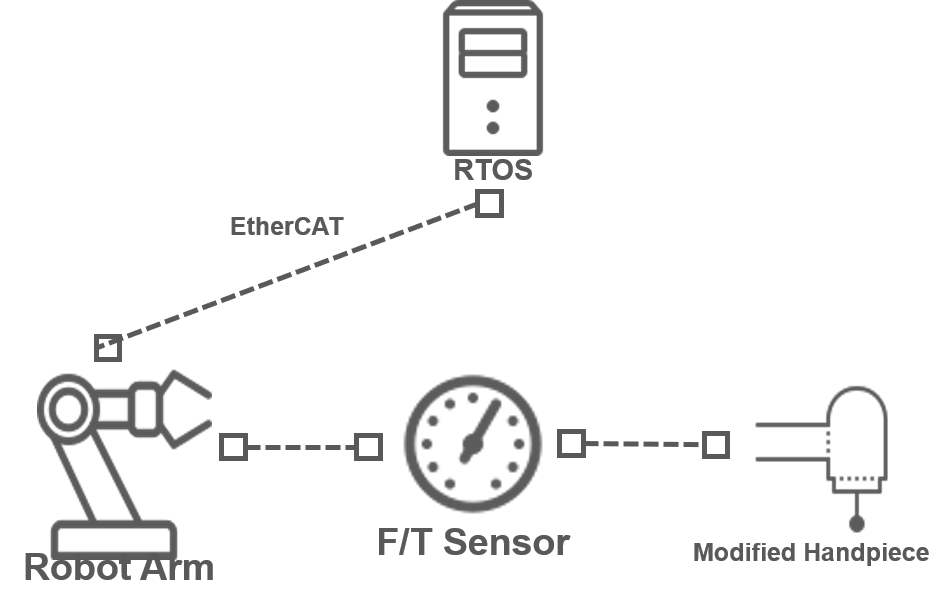
\includegraphics[width=0.7\linewidth]{Images/EtherCAT.png}
\caption{Communication protocol -- EtherCAT. Master device is RT-target and slave devices are robot arm, F/T sensor and modified handpiece.}
\end{center}
\end{figure}
\label{fig:EtherCAT}
\begin{figure}[htbp]
\begin{center}
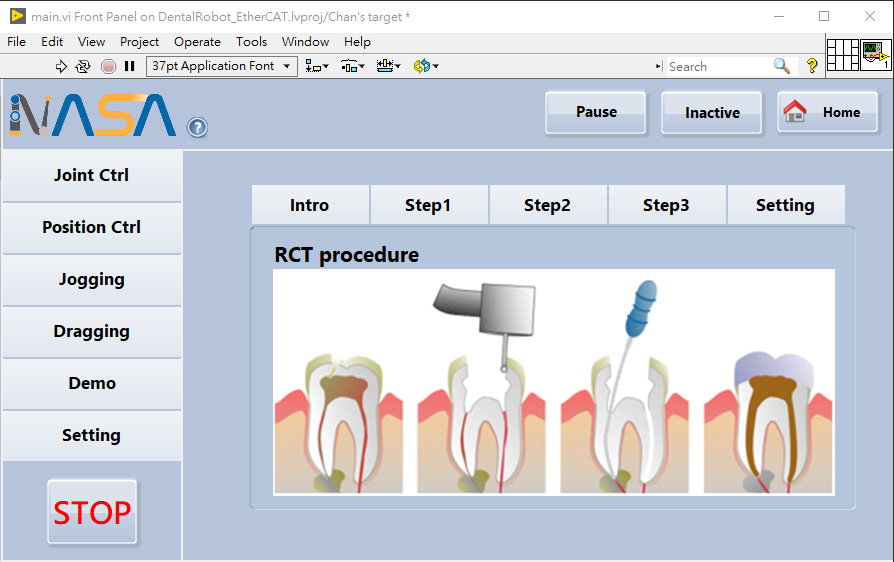
\includegraphics[width=1\linewidth]{Images/GUI.png}
\caption{Graph user interface with LabVIEW 2018}
\label{fig:GUI}
\end{center}
\end{figure}
\subsubsection{Hardware Setup}
\vspace{-5mm}
\hspace*{6mm}In Figure \ref{fig:system}, a motion capture system -- Impulse X2E (PhaseSpace, San Leandro, CA) is incorporated to obtain the handpiece and root positions . There were four cameras with high resolution sensor around the robot and their resolutions are around $1$ mm. The motion capture system can capture LEDs and calculate their Cartesian position for $960$ frames per second. Moreover, a Stewart platform on which a root acrylic model is mounted is set up to simulate a small patient moving. 
\begin{figure}[htbp]
\begin{center}
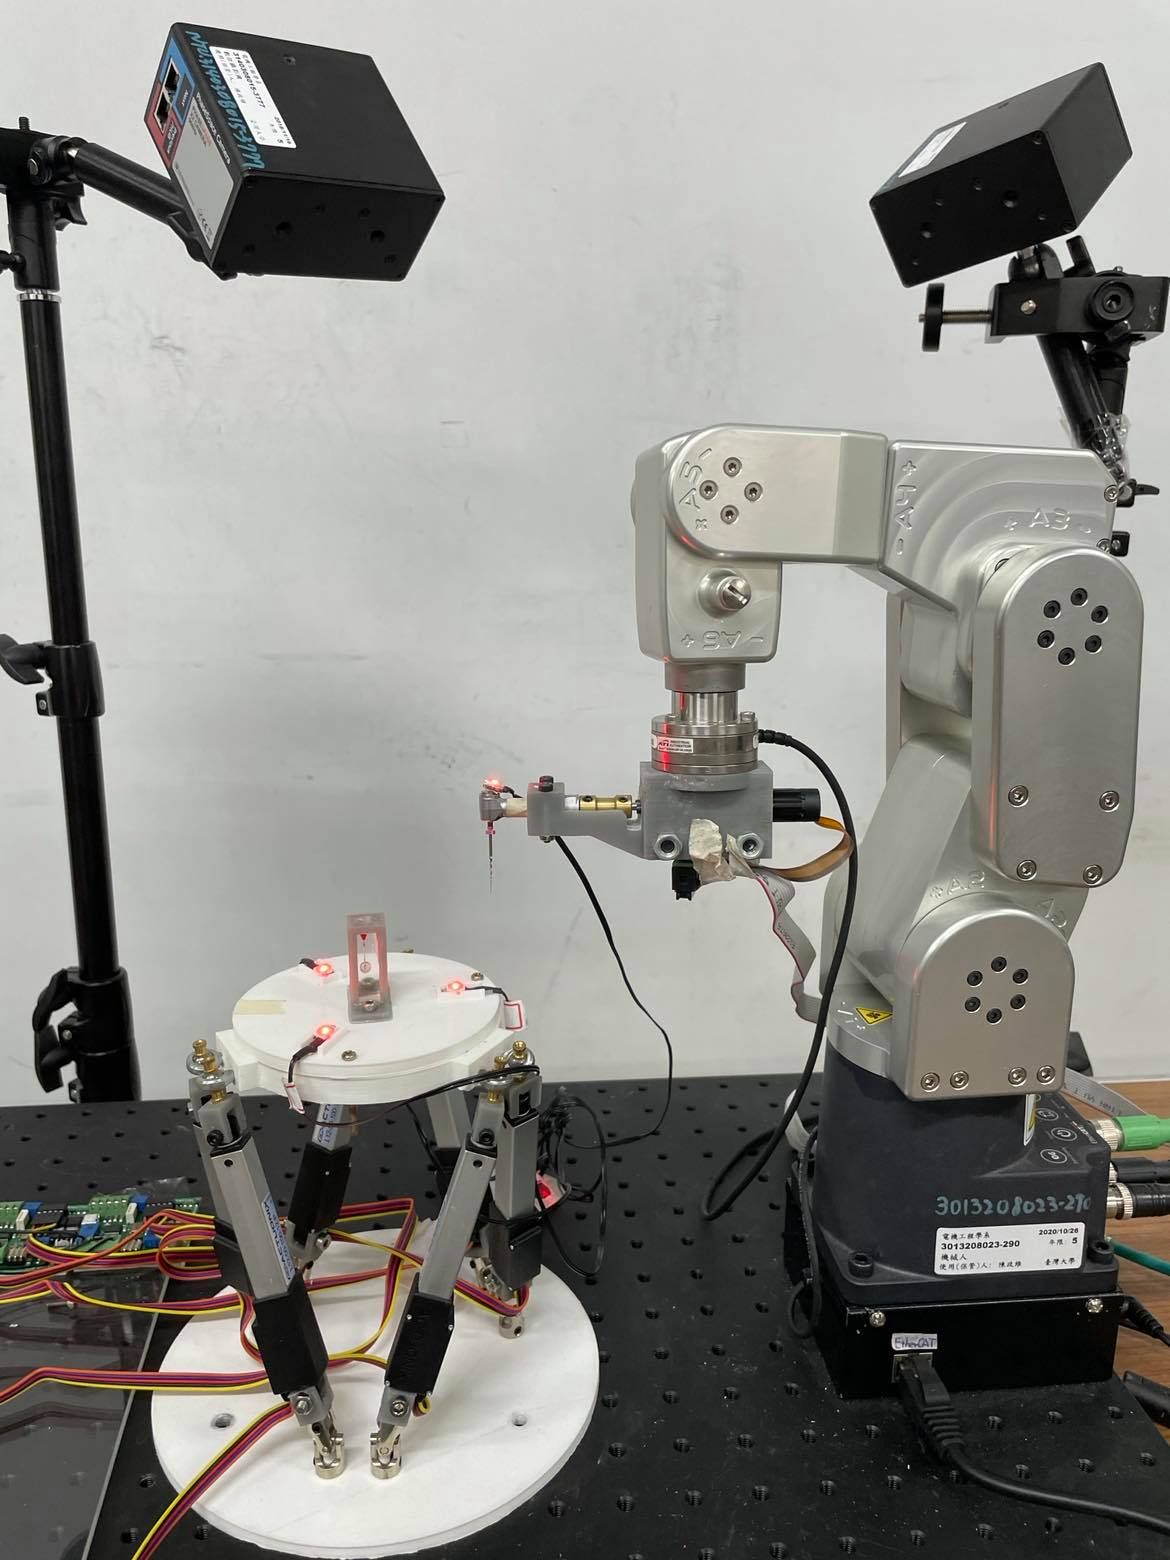
\includegraphics[width=0.6\linewidth]{Images/System.jpg}
\caption{Experimental setup with DentiBot, a motion-capture system capturing LEDs, and a Stewart platform simulating patient moving}
\label{fig:system}
\end{center}
\end{figure}
\par
To record the handpiece and root positions, a LED marker is located on the driller and the other three LED markers forming a equilateral triangle are seated on the Stewart platform. Therefore, the handpiece position is directly obtained and the root position is calculated as following equation
\begin{equation*}
\begin{split}
p_{root} = \frac{p_{1} + p_{2} + p_{3}}{3}
\end{split}
\end{equation*}
where $p_{root}$ denotes the root position and $p_{i}$ denote the positions of LEDs obtained from the motion capture system. 
\par
Also, the positions related to the motion capture system frame are transformed to the Stewart platform frame. Note that there is an original offset of around $55$ mm in the vertical direction between the root and handpiece in this setup. This original offset magnifies the relative distance on the X-axis and Y-axis. Also, An inaccurate 3-D print support used to stick three LEDs and acrylic roots lead to wrong centroid point and position biases. The flexible property of endodontic files absorbs contact forces and delays respond time. The root acrylic model has drilled thoroughly by a file and forms a cone shape in advance. Therefore, there is an another bais between the root and the endodotic file. Besides, if the motion capture system captures a LED with less than three cameras, the position information will be incorrect. To obtain stable data, four cameras are set up around DentiBot and the Stewart platform. Therefore, there are many factors to affect the position result and should be in afterward discussion.
\newpage
The specifications of the hardware and software environment set in the experiments are listed in Table \ref{tab:exp_specification}. The detail specifications of the robot arm and F/T sensor are shown in Table \ref{tab:meca_specification} and Table \ref{tab:mini40_specification}.

\begin{table}[htbp]
\centering
\tabcolsep=20pt
\arrayrulewidth=1pt
\caption{Specifications of the hardware and software environments}
\label{tab:exp_specification}
\par
\begin{tabular}{|c|c|} 
\hline
\rowcolor{lightgray!40}Item						&Specification				\\	\hline
Development Environment							&LabVIEW 2018					\\	\hline
\multirow{2}{*}{Real-Time Operating System}		&National Instrument-RT target	\\
												&CPU: Intel Core 8				\\	\hline
Communication Protocol							&EtherCAT						\\	\hline
Robot Arm										&Mecademic-Meca500				\\	\hline
F/T Sensor										&ATI-Mini40						\\	\hline
\multirow{2}{*}{Handpiece Motor}							&Maxon - servo motor				\\
												&Gear ratio: 67					\\	\hline
\multirow{2}{*}{Motion Capture System}			&PhaseSpace-Impulse X2E 		\\
												&Resolution: 1mm				\\	\hline
Stewart Platform								&Actuoanix - Linear Actuator				\\	
\hline
\end{tabular}
\end{table}

\begin{table}[htbp]
\centering
\tabcolsep=18pt
\arrayrulewidth=1pt
\caption{Technical specifications of the robot arm - meca500}
\label{tab:meca_specification}
\par
\begin{tabular}{|>{\columncolor{lightgray!20}}c|l|} 
\hline
Payload						&$0.5$ kg					\\	\hline
Repeatability				&$0.005$ mm					\\	\hline
Reach (at wrist center)		&$260$ mm	\\ \hline
Total weight				&$4.5$ kg						\\	\hline
\multirow{6}{*}{}Joint range&joint 1: $-175^\text{o}$ to $+175^\text{o}$				\\	
							&joint 2: $-70^\text{o}$ to $+90^\text{o}$				\\	
							&joint 3: $-135^\text{o}$ to $+70^\text{o}$				\\	
							&joint 4: $-170^\text{o}$ to $+170^\text{o}$				\\	
							&joint 5: $-115^\text{o}$ to $+115^\text{o}$				\\	
							&joint 6: $\pm 100$ revolutions				\\	\hline
Speed of joints 1–6 &${150, 150, 180, 300, 300, 500}$ $^\text{o}\text{/s}$				\\	\hline
Brakes 				&On joints 1, 2 and 3				\\	\hline
Robot mounting 		&Any orientation				\\	\hline
Safety module		&Category 3, PL d				\\	\hline
Power supply 		&90-264 VAC, 50-60 Hz (in) / 24 VDC (out)				\\	\hline
Communication 		&TCP/IP, EtherCAT, Ethernet/IP				\\	\hline
Controller 			&Embedded in robot base				\\	\hline
Protection rating 	&IP 40								\\	
\hline
\end{tabular}
\end{table}

\begin{table}[htbp]
\centering
\tabcolsep=10pt
\arrayrulewidth=1pt
\caption{Technical specifications of the F/T sensor - mini40}
\label{tab:mini40_specification}
\par
\begin{tabular}{|>{\columncolor{lightgray!20}}c|l|} 
\hline
Weight										&0.0499 kg	\\  \hline
Diameter									&40 mm  	\\ 	\hline
Height										&12.2 mm 	\\	\hline
\multirow{4}{*}{}Sensing range					&Fx,Fy: 20 N\\
											&Fz: 60 N\\
											&Tx,Ty: 1 Nm\\	
											&Tz: 1 Nm\\	\hline
\multirow{4}{*}{}Resolution						&Fx,Fy: 1/100 N	\\
											&Fz: 1/50 N\\
											&Tx,Ty: 1/4000 Nm\\	
											&Tz: 1/4000 Nm\\	\hline										
\multirow{4}{*}{}Single-axis overload 			&Fxy: ±810 N  \\	
											&Fz	±2400 N  \\
											&Txy	±19 Nm  \\
											&Tz	±20 Nm  \\ \hline
\multirow{4}{*}{}Stiffness (calculated)   		&X-axis \& Y-axis forces (Kx, Ky): 1.1x107 N/m   \\	
											&Z-axis force (Kz): 2.0x107 N/m   \\	
											&X-axis \& Y-axis torque (Ktx, Kty): 2.8x103 Nm/rad   \\	
											&Z-axis torque (Ktz): 4.0x103 Nm/rad   \\	 \hline
\multirow{2}{*}{}Resonant Frequency 			&Fx, Fy, Tz: 3200 Hz  \\
											&Fz, Tx, Ty: 4900 Hz  \\
\hline
\end{tabular}
\end{table}

\newpage
\section{Force-Guided Alignment}
\hspace*{6mm}The aim of this experiment was to validate the feasibility of force-guided alignment and patient tracking while drilling, we set up three experiments with different scenarios. The metric was to check whether it was possible that DentiBot inserted an endodontic file into a small root and confronted a patient moving at the same time.
\begin{figure}[htbp]
\begin{center}
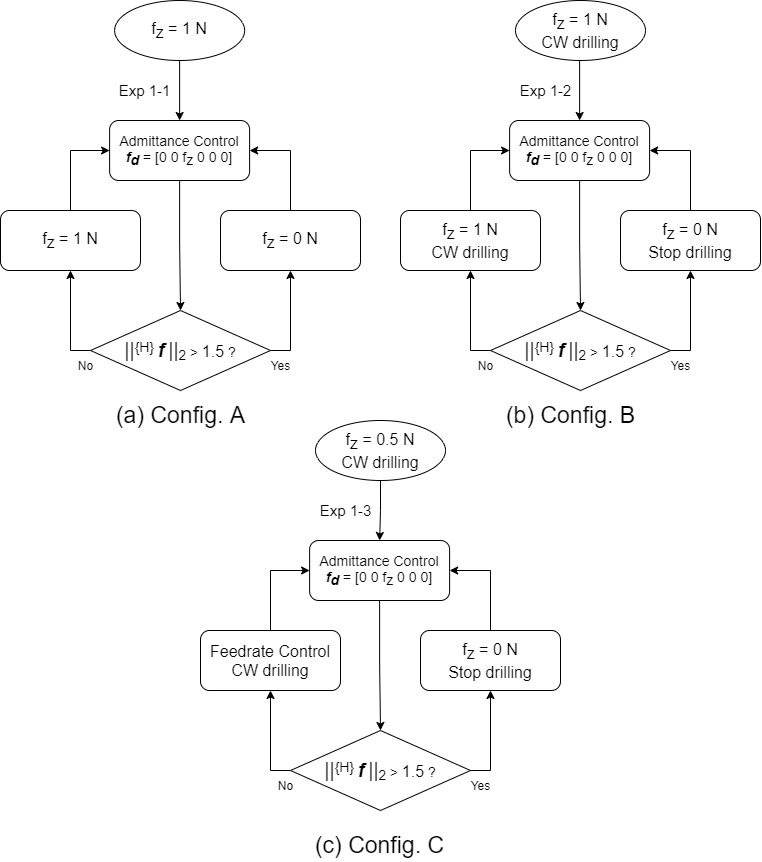
\includegraphics[width=1\linewidth]{Images/Exp1_motion planning.png}
\caption{Flow charts for force-guided alignment experiment. (a) shows Config.A -- inserting without file rotation. (b) shows Config.B --  inserting with file rotation. (c) shows Config.C --  inserting with file rotation and file feedrate control.}
\label{fig:exp_motion planning}
\end{center}
\end{figure}
\par	
Three experiment were designed with three configurations listed below and shown in Figure \ref{fig:exp_motion planning}.

\begin{enumerate}
\item[] Config. A -- Inserting without file rotation
\item[] Config. B -- Inserting with file rotation
\item[] Config. C -- Inserting with file rotation and file feedrate control
\end{enumerate}
\par
To simulate a patient moving, a Stewart platform with six degrees of freedom was incorporated.  When the patient moved to a point, our system should move to the same place. Therefore, the target and handpiece positions would be compared to check if our system tracked the patient or not. PhaseSpace - Impulse X2E, a motion capture system, was involved in obtaining the above positions in real-time. 
\par
The Stewart platform was scheduled for motion planning. It would move to (0, 0, 0), (15, 0, 0), (15, 0, 15), (0, 0, 15) related to Stewart frame. These points formed a $15*15$ mm square composed of two horizontal and two vertical lines. The command position trajectory is illustrated in Figure \ref{fig: position command}. The Stewart platform is planned to go along with a square at $3$ mm/s first, then stop for $10$ seconds, then go along with a square at a faster velocity, and so on. The velocities of four rounds are $3$ mm/s, $4$ mm/s, $5$ mm/s, and $6$ mm/s. Each cycle took $20$, $15$, $12$, $10$ seconds separately and total experiment time was $87$ seconds. Note that in reality linear interpolation was implemented to command the Stewart platform. The motion of the Stewart platform was received $4 \times 100$ steps and executed at an equally distributed time. Even though these $4$ points were cut to $400$ points and then calculated by inverse kinematics. The X-axis motion had an apparent distortion due to the hardware.
\begin{figure}[htbp]
\begin{center}
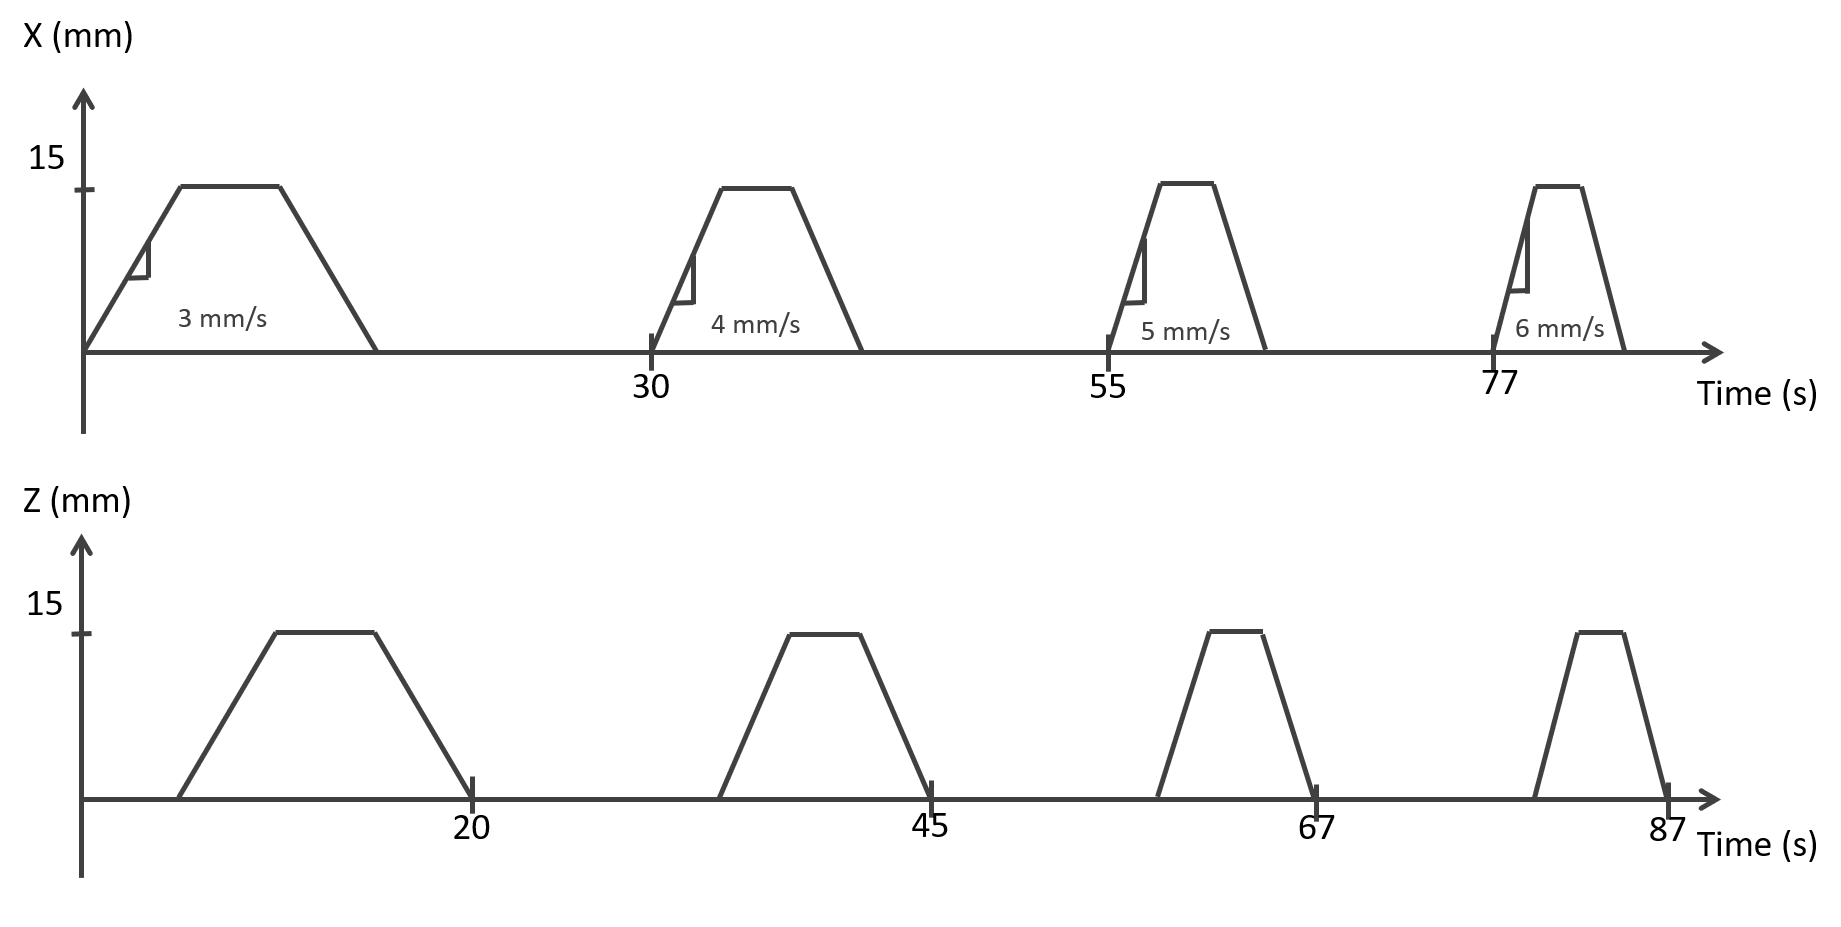
\includegraphics[width=1\linewidth]{Images/position command.png}
\caption{Position command of Stewart platform for force-guided alignment experiment}
\label{fig: position command}
\end{center}
\end{figure}	
\par
Parameters setting of admittance control in Experiment 1 is shown in Table \ref{tab: para_adm_exp1}. The parameter diagonal matrix $\mathbf{K}$ is proportional to the gain and $\mathbf{B}$ is inversely proportional to the gain. Therefore, the same values is set in all experiment except $b_6$. $b_6$ is relevant to the rotation along with Z-axis. The rotation along with Z-axis driven by the robot arm should be deactivated in Config. A and B because the file rotation is driven by the motor. If the rotation along with z-axis is on duty and the file is drilling, the robot arm would rotate along with Z-axis in opposite direction. Hence, $b_6$ is set a infinite value to deactivate the rotation along with Z-axis. Config. C is the last technical experiment and is designed as pre-clinical task, but the metrics are still same as the previous experiment. Because a slow inserting is required when performing the endodontic treatment. Therefore, the maximum value of $f_z$ was set $0.5$ in Config. C to limit the the highest velocity. 
\par
\begin{table}[htbp]
\centering
\tabcolsep=22pt
\caption{Parameters setting of admittance control in Experiment 1.}
\label{tab: para_adm_exp1}
\begin{tabular}{cccc} 
\hline \hline
Parameter	&Config. A	&Config. B	&Config. C			\\
\hline
$k$			&$500$		&$500$		&$500$				\\
$f_z$		&$1$		&$1$		&$-0.2 \sim 0.5$	\\
$b_1$		&$80$		&$80$		&$80$				\\
$b_2$		&$80$		&$80$		&$80$				\\
$b_3$		&$80$		&$80$		&$80$				\\
$b_4$		&$80$		&$80$		&$80$				\\
$b_5$		&$80$		&$80$		&$80$				\\
$b_6$		&$80$		&$\infty$	&$\infty$			\\
\hline
\multicolumn{4}{c}{ $\mathbf{K} = \text{diag}(k,k,k,k,k,k), \mathbf{B} = \text{diag}(b_1,b_2,b_3,b_4,b_5,b_6)$} \\
\hline\hline	
\end{tabular}
\end{table}
\subsubsection{Results}
\hspace*{6mm} There were three metric types of figures to show the results of Config. A, B, and C listed as following.
\begin{enumerate}
	\item The position of handpiece and root and their relative distance
	\item The force vs the velocity
	\item The force vs the handpiece position
\end{enumerate}
\hspace*{6mm}An imperative metric was whether the robot could move as the root moved. Therefore, the first figure was the position information. The position of handpiece and root were compared with and the relative distance between them was evaluated. The left blue axis of the first figure was for the position of hadndpiece and root and the right red one was for the relative distance. Second, the input of admittance control was force vector and output was velocity vector. Hence, the force and the velocity were compared in the second figure. The left blue axis of the second figure was for the force and the right red one was for the command velocity and real velocity. Last, the force and the position of robot were compared in the third figure. The left blue axis of the third figure was for the force, and the right red one was for the position of robot. Note that the real position and velocity data were transformed from the PhaseSpace frame to the Stewart platform frame. The force information were also transformed to the Stewart platform frame from the handpiece frame. Therefore, all data were all considered in the Stewart frame.
\begin{figure}[htbp]
\begin{center}
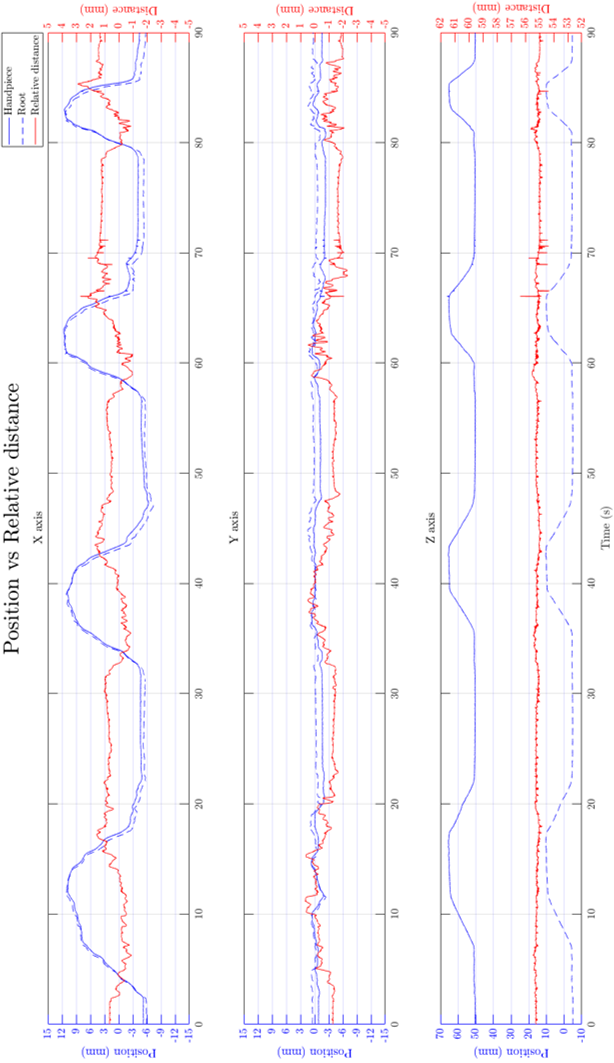
\includegraphics[width=0.9\linewidth]{Images/exp/exp1_1_1.png}
\caption{Config. A: Handpiece position vs root position root and their relative distance}
\label{fig: exp1_1_1}
\end{center}
\end{figure}	
	
\begin{figure}[htbp]
\begin{center}
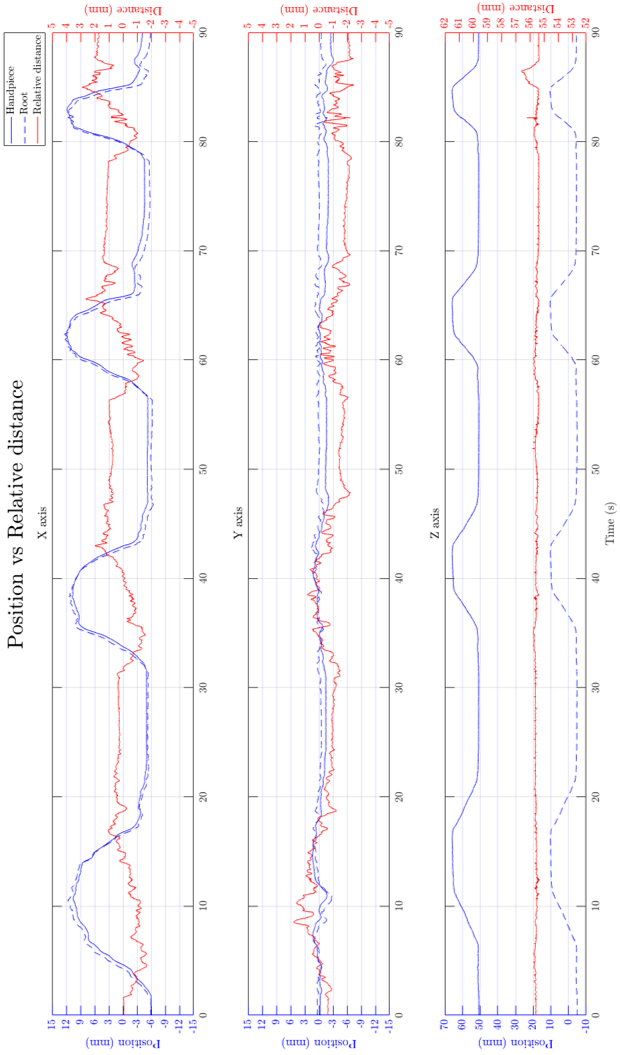
\includegraphics[width=0.9\linewidth]{Images/exp/exp1_2_1.png}
\caption{Config. B: Handpiece position vs root position root and their relative distance}
\label{fig: exp1_2_1}
\end{center}
\end{figure}	
			
\begin{figure}[htbp]
\begin{center}
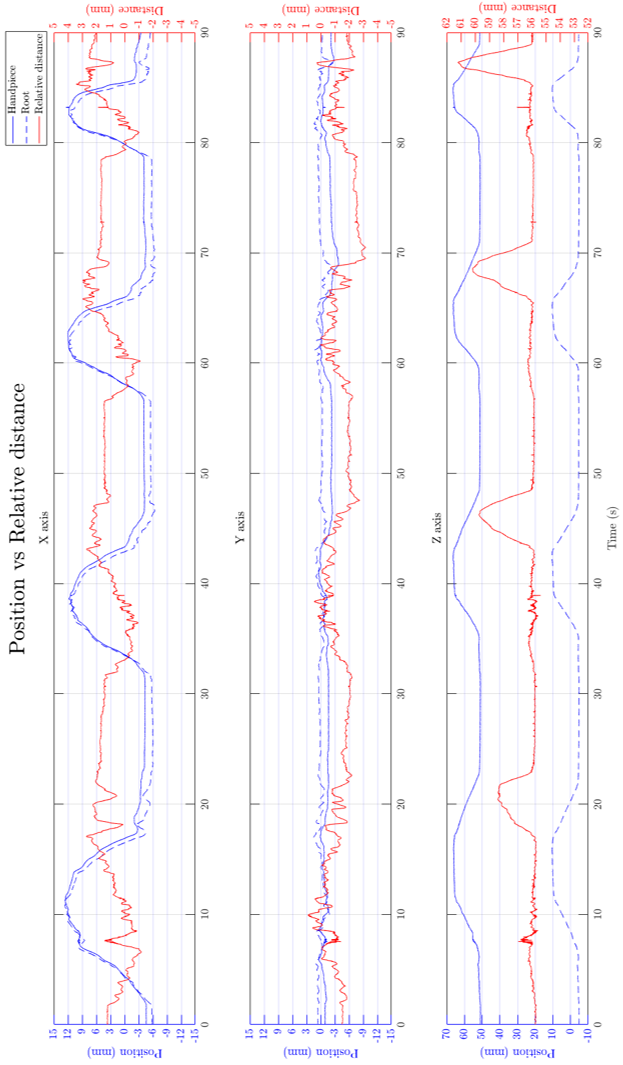
\includegraphics[width=0.9\linewidth]{Images/exp/exp1_3_1.png}
\caption{Config. C: Handpiece position vs root position root and their relative distance}
\label{fig: exp1_3_1}
\end{center}
\end{figure}		

\par
The first metric type of figure is the position of handpiece and root and their relative distance. Config A, B, and C were plotted in Figure \ref{fig: exp1_1_1}, Figure \ref{fig: exp1_2_1}, and Figure \ref{fig: exp1_3_1} and were discussed together here. First, the trajectory of the Stewart platform was analyzed. Distortion of platform moving occurred and led to difference to the position command of Stewart platform shown in Figure \ref{fig:  position command}. Figure \ref{fig: distortion} shows the real platform moving simulated by the Stewart platform.
\begin{figure}[htbp]
\begin{center}
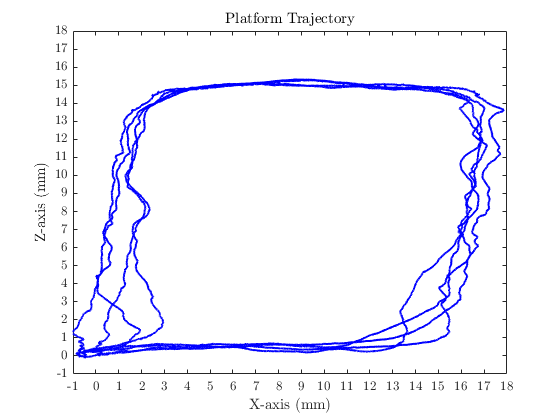
\includegraphics[width=0.8\linewidth]{Images/exp/platform moving.png}
\caption{Patient trajectory simulated by Stewart platform }
\label{fig: distortion}
\end{center}
\end{figure}	
\par
There was a apparent distortion around $3$ mm on X-axis when the platform was moving along with Z-axis. This distortion led to the fact that each cycle in the position plot on X-axis is not a trapezoid. The Stewart platform moving along with X-axis was smooth, so the position plot on Z-axis is a typical trapezoid. Therefore, the relative distance was calculated and became the most essential metric . 
\par
On X-axis we could find that there is a phase difference between the root position and the handpiece position. The main reason is that the file property is superelastic and delays the response time when the file bears a contact force. 
\par
Compared all X-axes and Y-axes from Config. A to C, the maximum relative distance are all around $3$ mm. This relative distance is acceptable because it came from many errors such as the motion capture system, the 3-D print support, and the flexible property of the endodontic file. On Z-axis, the maximum relative distance in Config.A approximately retains at $55$ mm; in Config. A and B, there is a ripple at around $87$th second. It is due to the file leaving out of the root when the platform was moving down along with Z-axis. The file chased the root because $f_z$ made DentiBot insert and the relative distance went back to the original offset after a few seconds. Why the file is easy to leave out of the root in Config. B and not in Config. A is the file rotation. As for Z-axis of Config. C, ripples were expected because the maximum $f_z$ was half of the previous. With the velocity is increasing, ripples are getting bigger. At $6$ mm/s velocity, the maximum relative distance is around $5$ mm. After around $5$ seconds, it could go back to the original offset.
\par
In conclusion, from Config. A to C, the maximum relative distances were all retained in an acceptable error. Despite that Config. C had a significant detachment between the endodontic file and the root, the file could track and go back to the original offset. It is worth noting that there is a distortion when the Stewart platform moves along with Z-axis, which means the force-guided alignment could track and compensate the surgical path in real-time with high performance.

\begin{figure}[htbp]
\begin{center}
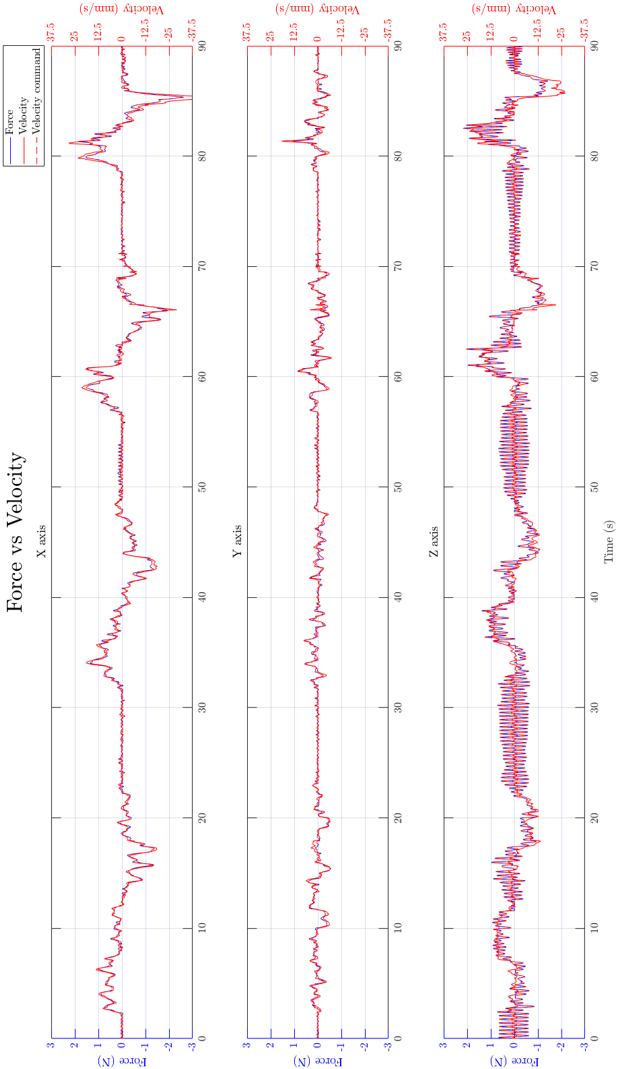
\includegraphics[width=0.9\linewidth]{Images/exp/exp1_1_2.png}
\caption{Config. A: Force vs Velocity and Velocity command}
\label{fig: exp1_1_2}
\end{center}
\end{figure}

\begin{figure}[htbp]
\begin{center}
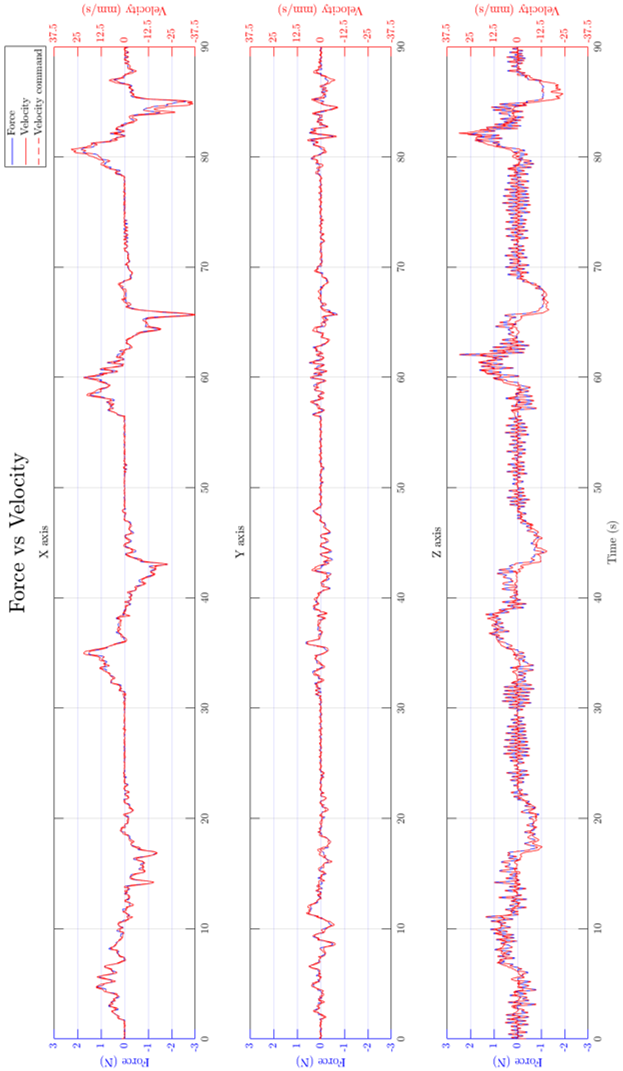
\includegraphics[width=0.9\linewidth]{Images/exp/exp1_2_2.png}
\caption{Config. B: Force vs Velocity and Velocity command}
\label{fig: exp1_2_2}
\end{center}
\end{figure}

\begin{figure}[htbp]
\begin{center}
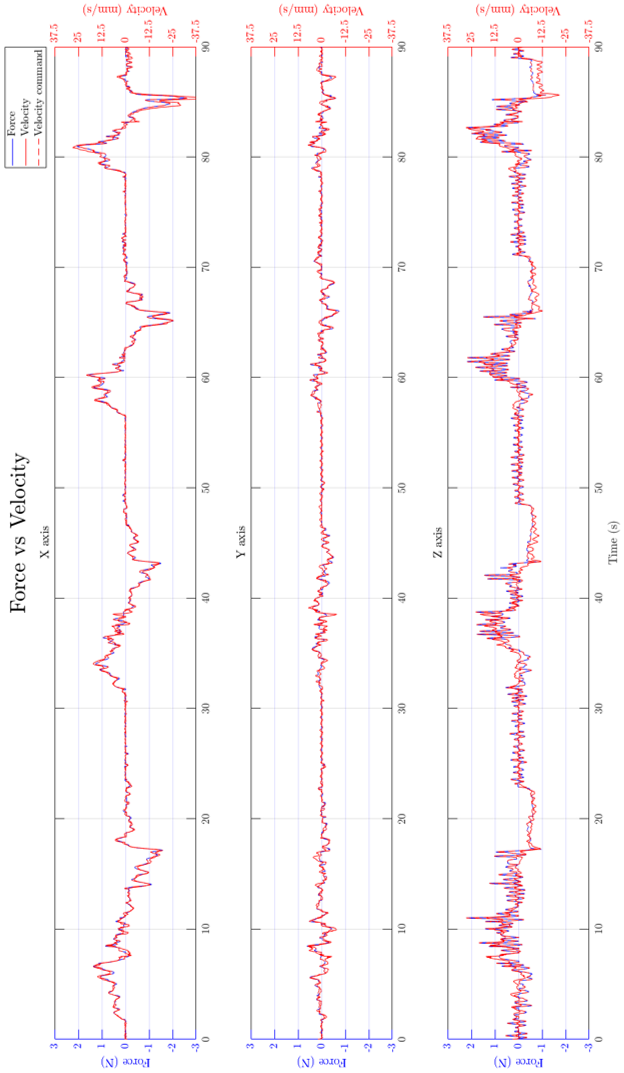
\includegraphics[width=0.9\linewidth]{Images/exp/exp1_3_2.png}
\caption{Config. C: Force vs Velocity and Velocity command}
\label{fig: exp1_3_2}
\end{center}
\end{figure}

\par 
The second metric type of figure is comparing the detected force with the command velocity and the real velocity. Config. A , B, and C were plotted in Figure \ref{fig: exp1_1_2}, Figure \ref{fig: exp1_2_2}, and Figure \ref{fig: exp1_3_2} and were discussed together here. In theory, the force should match the command velocity and have a highly positive correlation to the real velocity. From Config. A to Config. C, three plots are similar, overall the results compared to the theory are all correct. However, two phenomenons occurred on Z-axis. The first phenomenon is that there is oscillation due to excessive velocity caused by a large value of $f_z$. Too fast velocity would produce excessive force than the desired force when the file contacts the root bottom and lead to an opposite move. The other phenomenon is zoomed in and shown in Figure \ref{fig: zoom_in}. The difference between the command and real velocity is caused by the detachment between root and file.

\begin{figure}[htbp]
\begin{center}
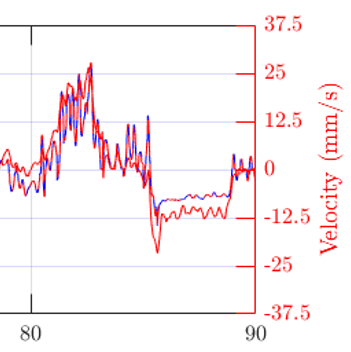
\includegraphics[width=0.6\linewidth]{Images/exp/zoom_in.png}
\caption{Zoom-in plot of Force vs Velocity on Z-axis from 80th to 90th second}
\label{fig: zoom_in}
\end{center}
\end{figure}



\begin{figure}[htbp]
\begin{center}
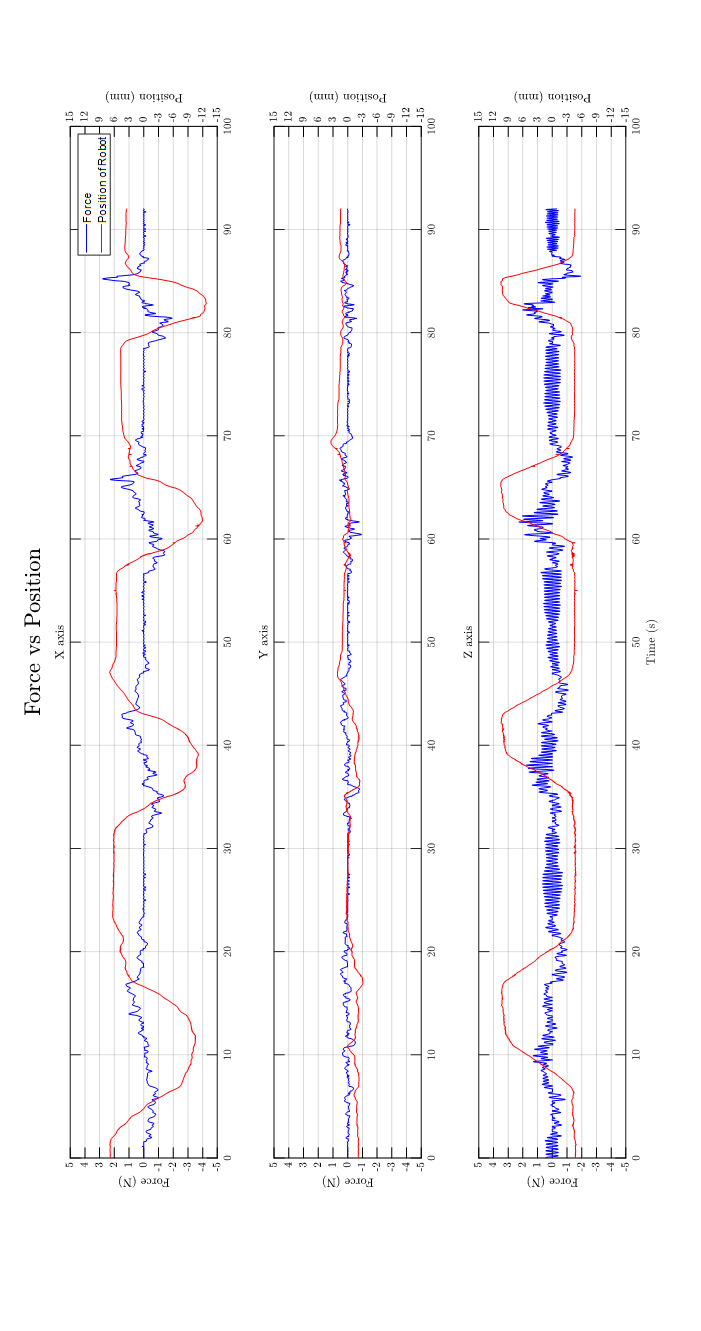
\includegraphics[width=0.9\linewidth]{Images/exp/exp1_1_3.png}
\caption{Config. A: Force vs Handpiece position}
\label{fig: exp1_1_3}
\end{center}
\end{figure}

\begin{figure}[htbp]
\begin{center}
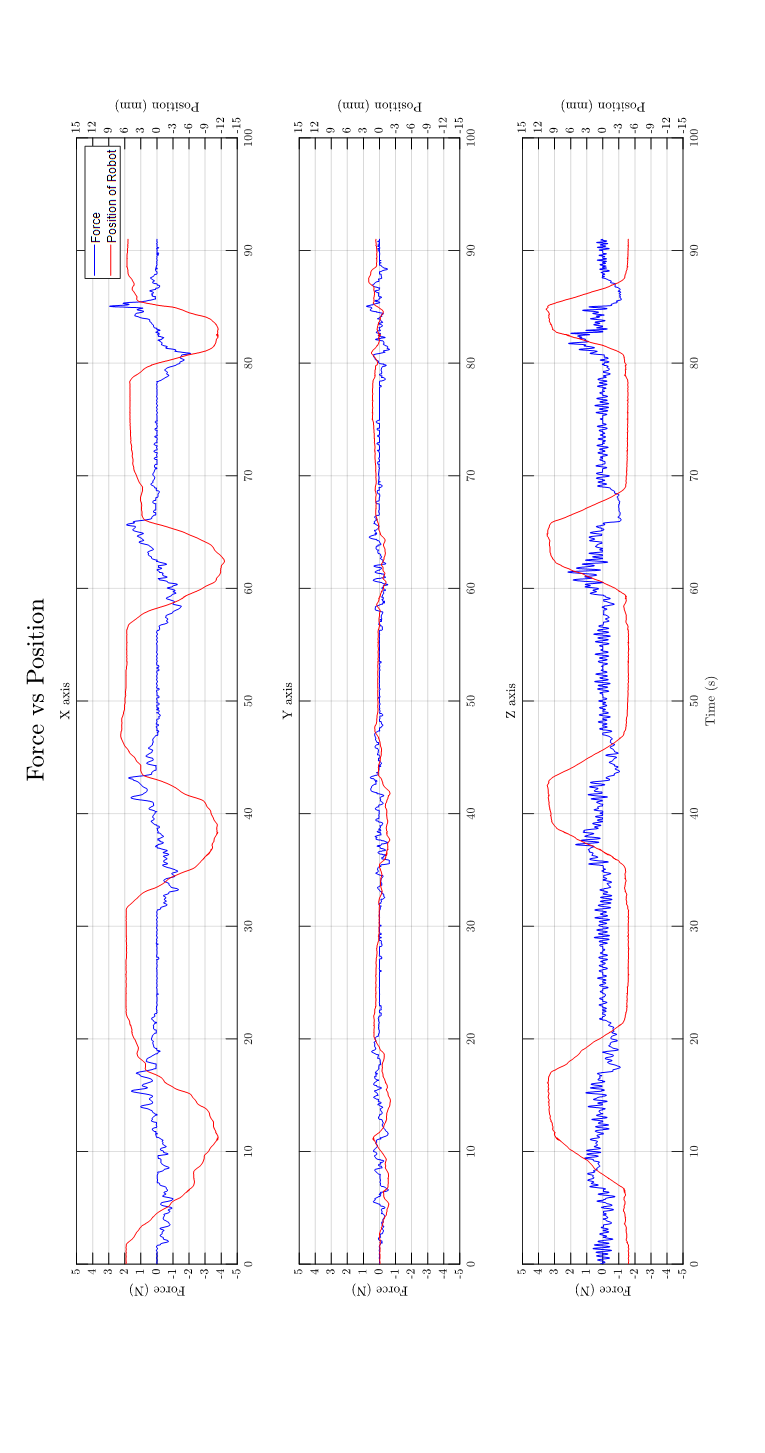
\includegraphics[width=0.9\linewidth]{Images/exp/exp1_2_3.png}
\caption{Config. B: Force vs Handpiece position}
\label{fig: exp1_2_3}
\end{center}
\end{figure}

\begin{figure}[htbp]
\begin{center}
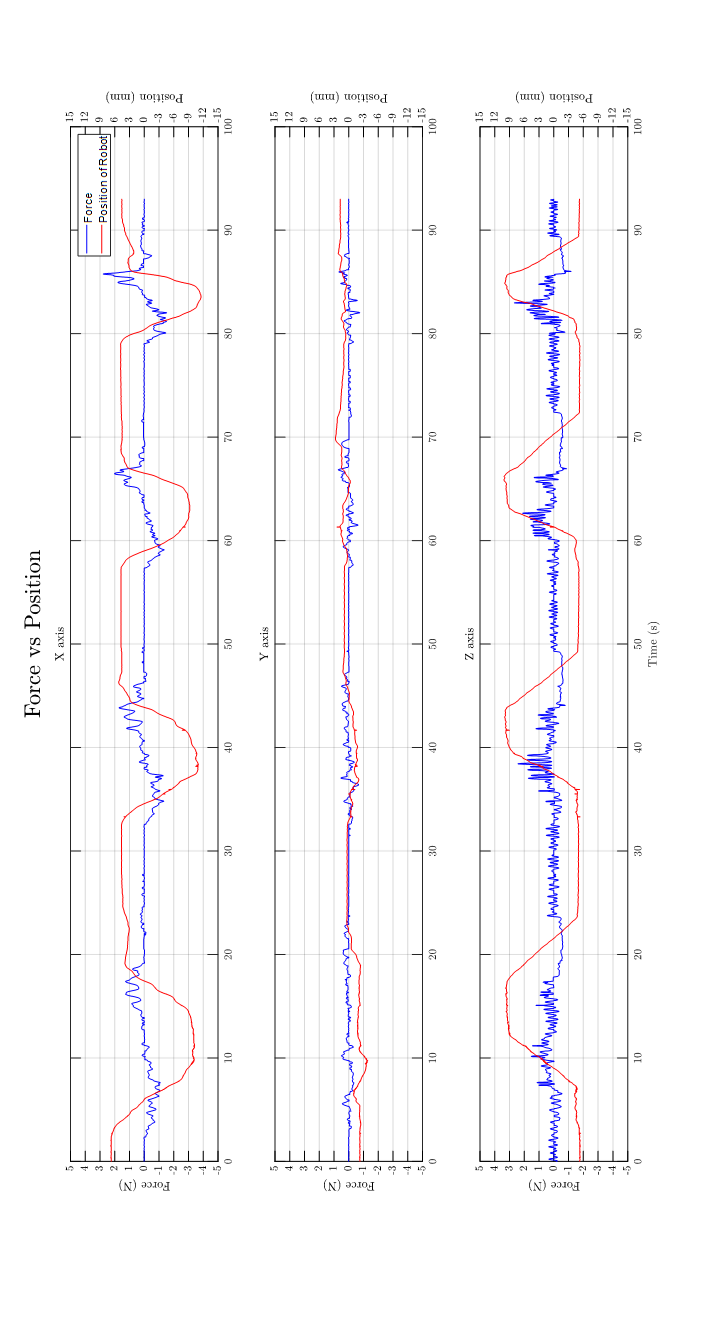
\includegraphics[width=0.9\linewidth]{Images/exp/exp1_3_3.png}
\caption{Config. C: Force vs Handpiece position}
\label{fig: exp1_3_3}
\end{center}
\end{figure}

\par
The third metric type of figure is comparing the detected force with the handpiece position. Config. A , B, and C were plotted in Figure \ref{fig: exp1_1_3}, Figure \ref{fig: exp1_2_3}, and Figure \ref{fig: exp1_3_3} and were discussed together here. An oscillation occurred on Z-axis is due to excessive velocity caused by a large value of $f_z$. A large value of $f_z$ means a faster inserting velocity. Once  the file contacts the bottom of root, the opposite force is produced and detected by the F/T sensor. The contact velocity is faster, then the opposite force is larger. Therefore, if the opposite force is larger than the desired force, DentiBot will move to the opposite direction. However, the opposite move will decrease the detected force and then make DentiBot move forward again. That is why the oscillation occurs.
\subsubsection{Conclusion of Force-Guided Alignment Experiment}
\hspace*{6mm}To conclude the experiment 1, the maximum relative distances on X-axis and Y-axis were all retained within $3$ mm. $3$ mm was an acceptable error because it could be the result of the inaccurate 3-D print support, the flexible property of endodontic files, and the motion capture system error. Despite that Config. C had a significant detachment between the endodontic file and the root, the file could track and go back to the original offset. Patient moving within $15$ mm is proved to be allowed because the force-guided alignment could track and compensate the surgical path in real-time with low error. Therefore, the experiment result has proved the feasibility of combining force-guided alignment, file feedrate control and patient tracking.

\newpage

\section{Pre-Clinical Evaluation}
\hspace*{6mm}We have verified the feasibility of combining force-guided alignment, file feedrate control. In what follows, an algorithm that combines all functions including force-guided alignment, patient tracking, inverse rotation control, and feed control were implemented in the pre-clinical trial as shown in Figure \ref{fig: exp2_motion planning}.
\begin{figure}[htbp]
\begin{center}
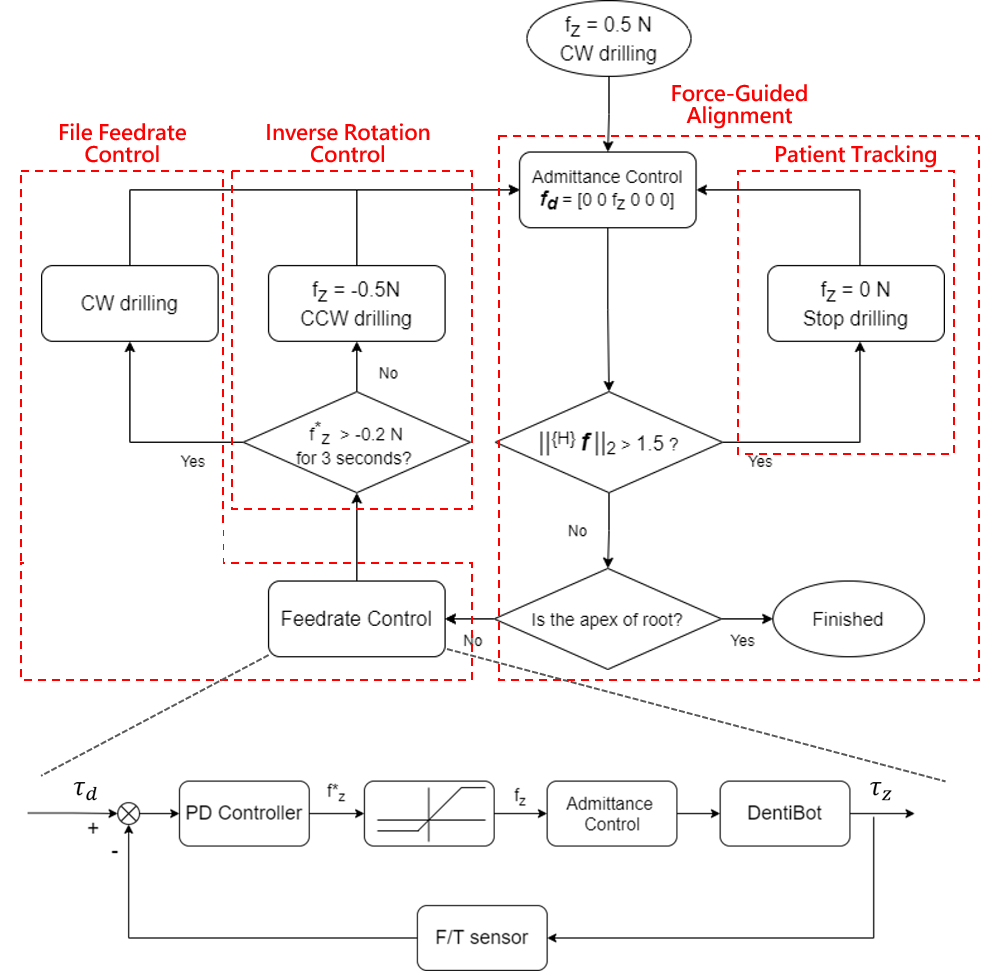
\includegraphics[width=1\linewidth]{Images/algorithm.png}
\end{center}
\caption{
Flowchart of the algorithm for autonomous endodontic treatment
}\label{fig: exp2_motion planning}
\end{figure}
\par
The metrics of the pre-clinical trial were completeness of root preparation and whether instrument fracture happened. To compare the completeness before and after the surgery, acrylic root phantoms were involved. The acrylic root phantoms were widely used in the operative technique classroom to simulate the clinical situations. Intern dentists practised the endodontic techniques with acrylic root phantoms. To simulate and visualize the pulp in roots, red pigment was filled with roots shown in Figure \ref{fig: root_single}. The top of the model is a cone shape and is not included to calculate the completeness because the cone area is not the drilling area. Therefore, the red line depicted in the figure is the calculated length. 
\par
Hence, completeness is defined as 
\begin{equation}
\begin{split}
	\text{Completeness} = \frac{R_b - R_a}{R_b} \times 100\%
\end{split}
\end{equation}
where $R_b$ denotes the red area before the treatment. $R_a$ denotes the remained red area after the treatment.
\begin{figure}[htbp]
\begin{center}
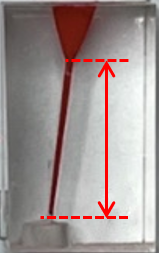
\includegraphics[width=0.15\linewidth]{Images/root_single.png}
\caption{Acrylic root phantom used in operative technique practice}
\label{fig: root_single}
\end{center}
\end{figure}
\par
Note that the acrylic root phantoms were all different due to manufacture process. Conditions of the acrylic root phantoms might be straight, titled, or even curve. 
\par
Six root models, A to F, were divided into two groups. The desired torque $\tau_d$ in file feedrate control was set $40$ and implemented in A, B, and C. On the other hand, $\tau_d$ was set $50$ in D, E, and F. Each model was treated for two times. The first round took $300$ seconds and the second round took $200$ seconds.
\subsubsection{Result}
\hspace*{6mm}In Figure \ref{fig: exp2_roots}, six root models before and after treatment are compared. There is few remained red pigment within roots. Besides, the roots were all shaped to cone shapes without ledging. Ledging is an irregular platform caused by an inappropriate operation such as too much force while drilling. Once ledging happens, it would impede the endodontic files to the apex. The results without ledging proved that force-guided alignment was effective to adjust the surgical path in real-time.
\begin{figure}[htbp]
\begin{center}
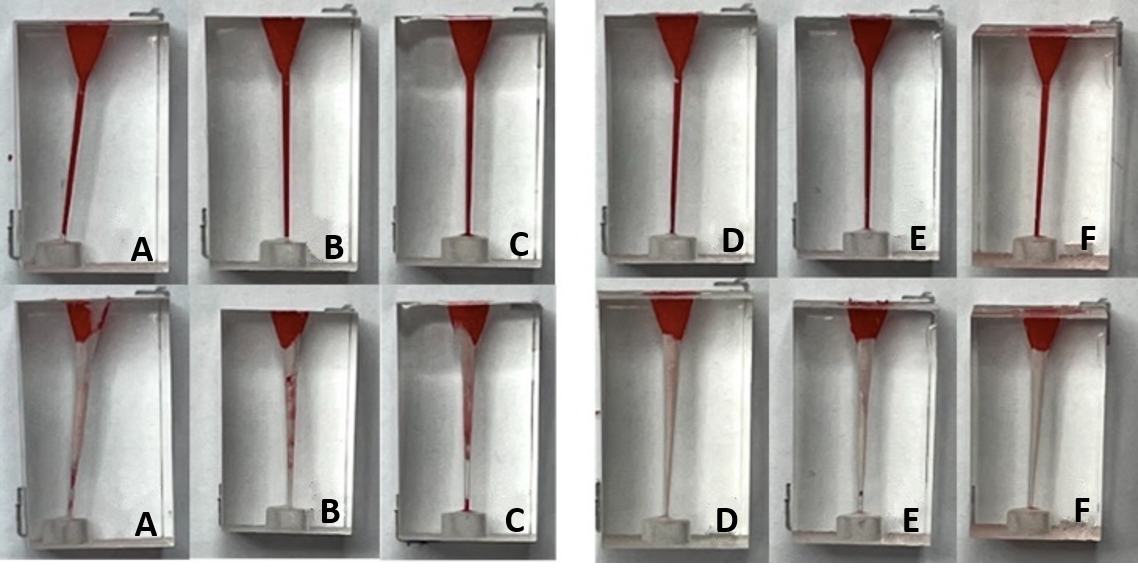
\includegraphics[width=0.9\linewidth]{Images/exp/roots.png}
\caption{Experiment 2: A comparison of completeness before and after two times drilling. $\tau_d$ were set 40 in A,B,C and 50 in D,E,F}
\label{fig: exp2_roots}
\end{center}
\end{figure}	
\par
To dissect the completeness, the root images were evaluated by image processing and shown in Table \ref{tab:pre-clinical}. The average completeness of A, B, C is $88.41\%$ and the average completeness of D, E, F is $99.2\%$. It means that $\tau_d\ 50$ below the maximum file bearing torque $62$ had higher completeness than  $\tau_d\ 40$. However, no matter $\tau_d$ was $40$ or $50$, it could both achieve high performance in root preparation and prevent instrument fracture.

\begin{table}[htbp]
\centering
%\tabcolsep=20pt
%\arrayrulewidth=1pt
\caption{Results of pre-clinical evaluation }
\label{tab:pre-clinical}
\begin{tabular}{ccccc} 
\hline \hline
\multirow{2}{*}{Number}	&Preoperative 		&Postoperative 		&\multirow{2}{*}{Completeness} 	&Instrument\\
						&Red Area (pixel)	&Red Area (pixel)	&								&Fracture	\\
\hline
A		&15652						&795						&94.92\%	&No\\
B		&17316						&2418						&86.04\%	&No\\
C		&17403						&2738						&84.27\%	&No\\
D		&16114						&53							&99.67\%	&No\\
E		&17047						&185						&98.91\%	&No\\
F		&18482						&180						&99.03\%	&No\\
\hline\hline
\end{tabular}
\end{table}
\subsubsection{Conclusion of pre-clinical evaluation}
\hspace*{6mm}In this experiment, the performance of root preparation using our robot was demonstrated. No ledging in all postoperative acrylic root phantoms proved that force-guided alignment could adjust the surgical path in real-time. Preoperative and Postoperative root models were evaluated their completeness and compared. The results verified the feasibility of robot-assisted endodontic treatment. 
